\chapter{User documentation}

In this chapter, we present an overview of the functionality of the application. The first section sketches out the overall
functionality of the application. The following sections describe each feature in more detail.

\section{Site map}

\section{Landing page}

The landing page displays a list of chants from a specified source, which is by default set to the provided data source \emph{CantusCorpus v0.2}.
As we assume that the number of all selected chants can be large, we do not display all of them at once. Instead, the user can choose the number of
chants displayed at once and paginate through the list to get to later ones.

The panel on the right side enables data source selection. To change data source (more than one can be selected at once), click the checkbox next
to the data source name and click \emph{save}. To hide or unhide the data source panel, click on the black \emph{Data sources} button. The panel
is available in the entire application.

\begin{figure}[!h]
\centering
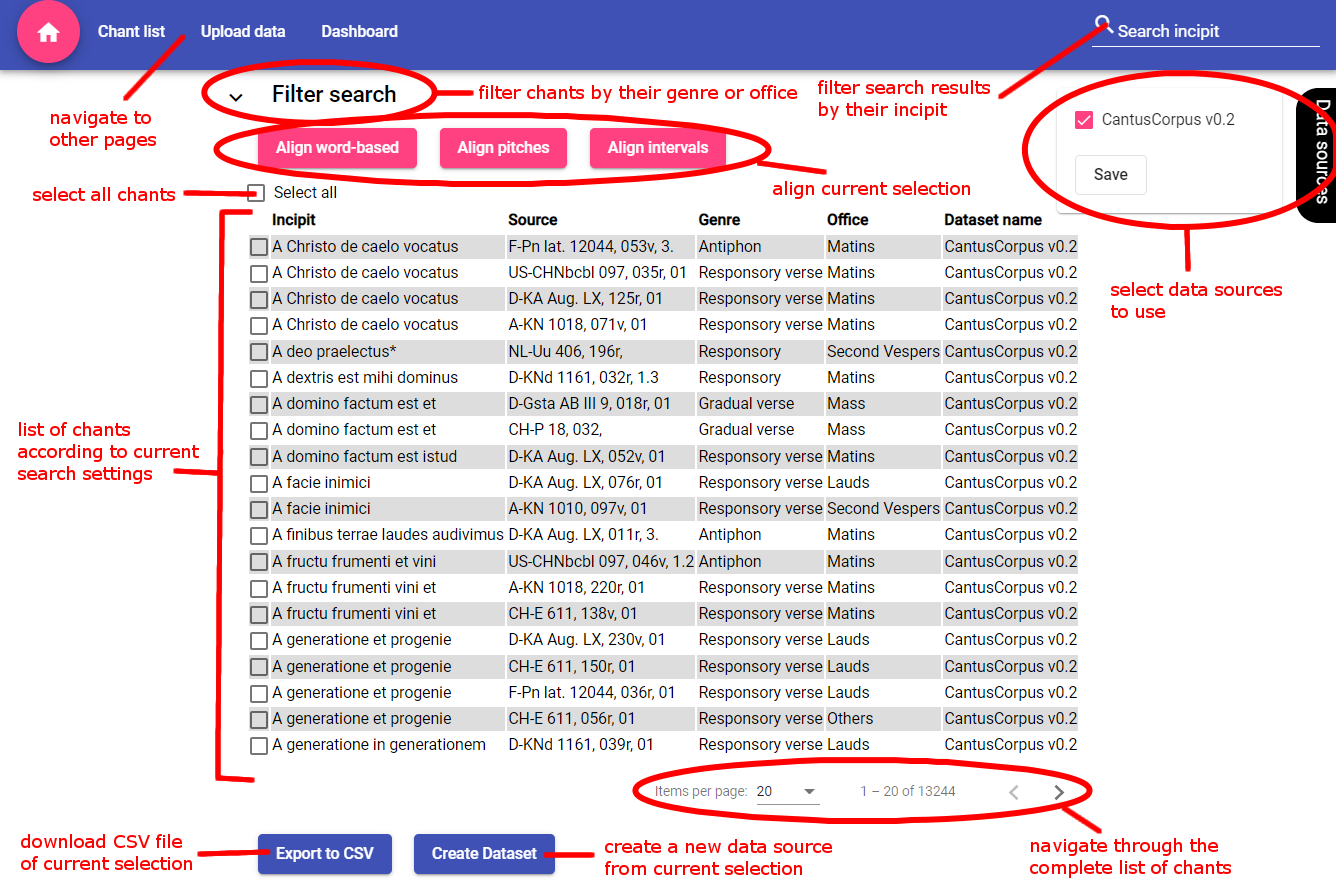
\includegraphics[scale=0.5]{udocs-homepage-marked}
\caption{Landing page and its features.}
\label{fig:land_page}
\end{figure}

\subsection{Incipit search}

The landing page provides the possibility to filter chants from the current selection by incipit. To do so, enter the desired string into
the field in the top-right corner marked as \emph{Search incipit} and press Enter. A set of chants that contain the query as a substring of their incipit will be displayed.
Be aware that a misspelled query will not return the correct results.

\begin{figure}[!h]
\centering

\includegraphics{udocs-search-incipit}
\caption{Entering search query into the \emph{Search incipit} box.}
\label{fig:inc-search}
\end{figure}

\begin{figure}[!h]
\centering
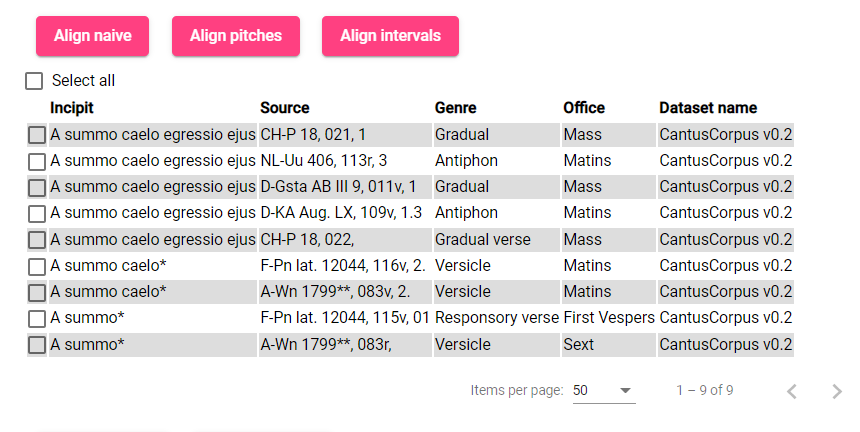
\includegraphics[scale=0.6]{udocs-after-incipit-search}
\caption{The result of the query. Notice that each incipit has the query as a substring.}
\label{fig:inc-search-result}
\end{figure}

\subsection{Search filter}

It is possible to filter the search results by their genre and office. The filter panel can be opened by clicking the down arrow next to the \emph{Filter search}
heading. By default, all genres and all offices are selected. To select or unselect some of them, click the checkbox next to their abbreviation. To select 
or unselect all genres or offices, click the checkbox next to \emph{All} in the respective section.

The filter panel does not use the full names of the genres and offices, as in some cases, the name can be very long. Instead, it uses their abbreviations as used 
in Cantus Index. Attachments XXX and YYY provide a list of genres, resp. offices and their abbreviations.

\begin{figure}[!h]
\centering
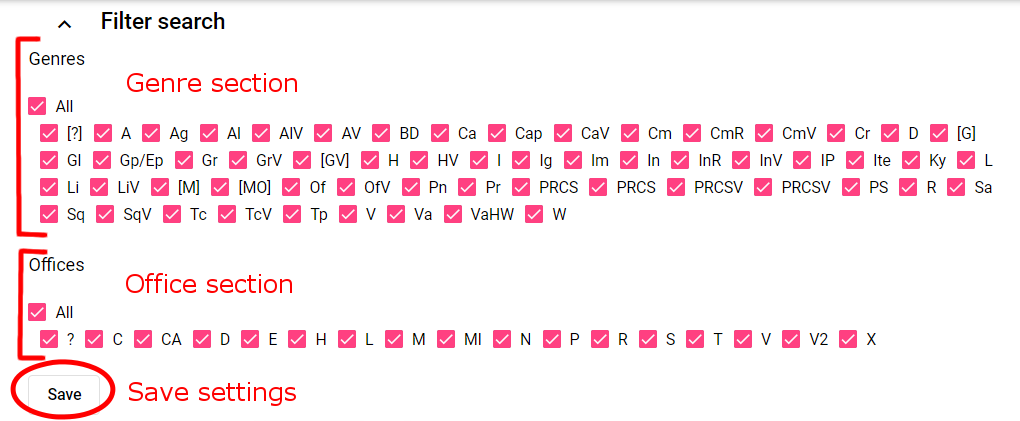
\includegraphics[scale=0.5]{udocs-filter-marked}
\caption{Search filter panel.}
\label{fig:search_filter}
\end{figure}

\subsection{Chant detail}

By clicking on a chant's incipit in the search results list, the user is redirected to a page which displays the chant's melody with the text in full,
as well as other information of interest. It shows the chant's Cantus ID, by which it can be found in the Cantus Database. It also shows a URL which
points to the corresponding entry on the Cantus website. These fields are valid for all chants from the default \emph{CantusCorpus v0.2} dataset,
but there is no guarantee of their correctness in user-uploaded data.

\begin{figure}[!h]
\centering
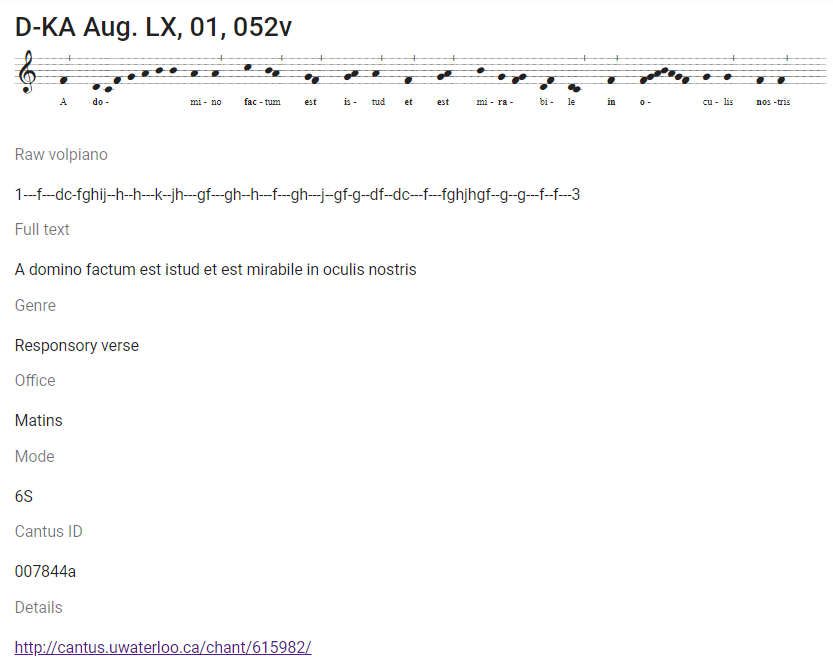
\includegraphics[scale=0.6]{udocs-chant-detail}
\caption{Page with the detail of the selected chant.}
\label{fig:chant-detail}
\end{figure}

\subsection{Data export}

The user may wish to export the results of their search into a CSV file. In that case, select the desired chants by checking the checkbox next to
their incipit (or \emph{Select all}) and click the \emph{Export to CSV} button at the bottom of the page. A file with the name \emph{dataset.csv}
will be automatically downloaded.

\begin{figure}[!h]
\centering
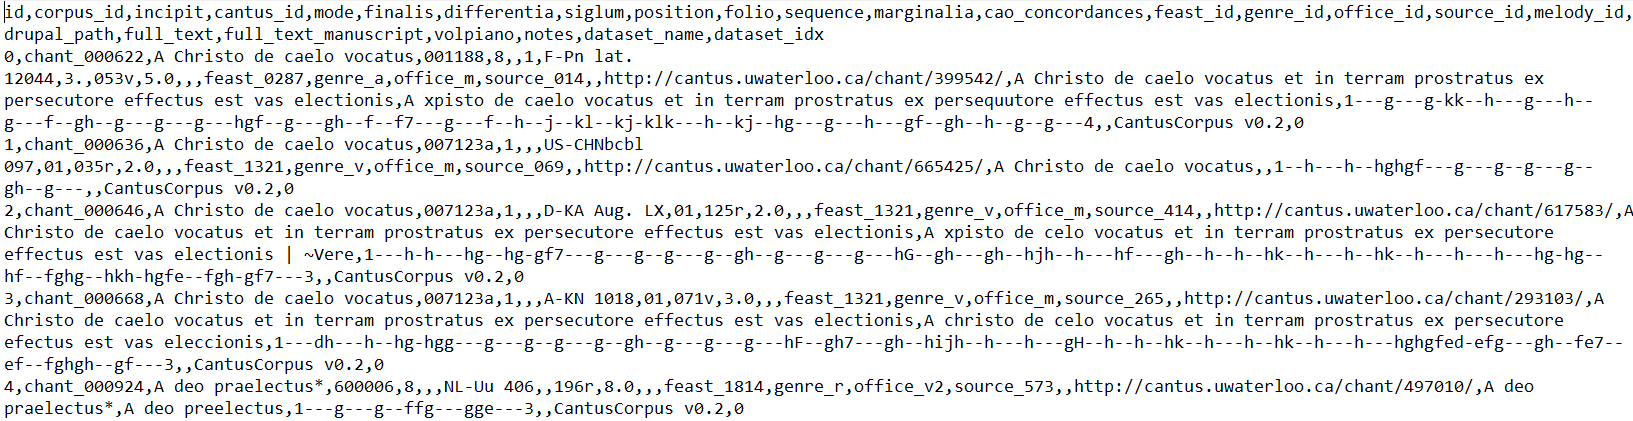
\includegraphics[scale=0.4]{udocs-exported-ds}
\caption{First few lines of the exported CSV file.}
\label{fig:export-ex}
\end{figure}

\section{Data source creation}

The application is not limited to the data present by default. The user can either create a data source from their search results, or upload
completely new data.

\subsection{Create from search}

To create a data source from the search results, check the checkboxes next to the desired chants and click the \emph{Create Dataset} button at the bottom
of the page. The user will be prompted for the data source name. If no name is entered, the name of the data source will be \emph{undefined}. After confirming
the name, the data source list will be automatically updated with the newly-created one.

\begin{figure}[!h]
\centering
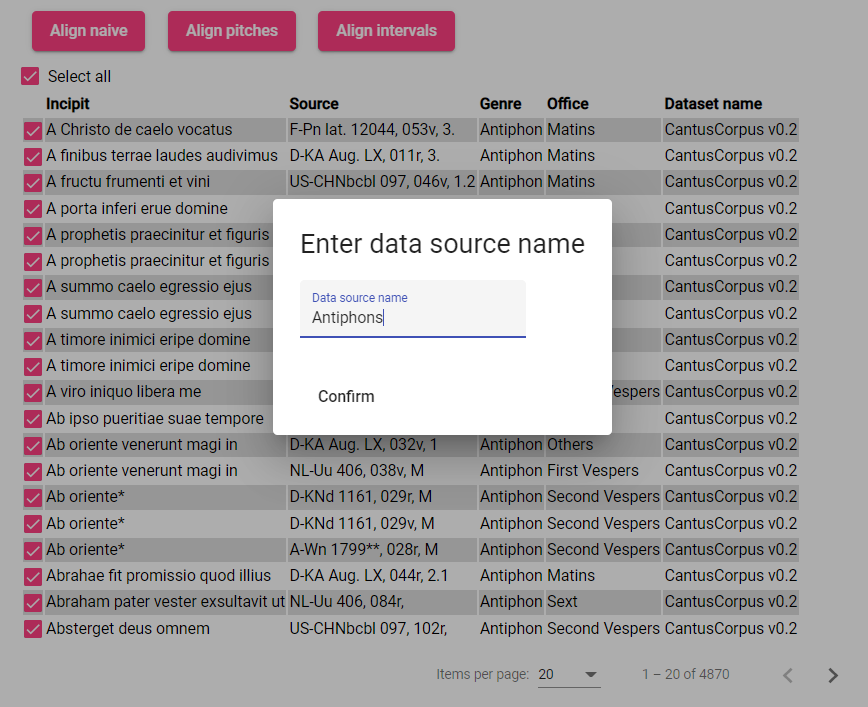
\includegraphics[scale=0.6]{udocs-create-ds}
\caption{Prompt for entering the name of the data source appears after clicking the \emph{Create Dataset} button.}
\label{fig:create-ds}
\end{figure}

\begin{figure}[!h]
\centering
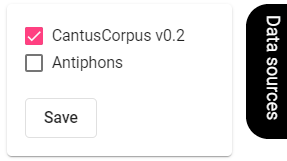
\includegraphics{udocs-ds-in-list}
\caption{The newly created data source automatically appears in the data source list.}
\label{fig:update-ds-antiphons}
\end{figure}

\subsection{User data upload}

To upload new data, navigate to the \emph{Upload data} page in the top panel. Select the file to upload and enter the data source name. The file should be
in CSV format and its contents are specified in section XXX. Click \emph{Upload} to upload the file. After the file is processed, the data source list will
be automatically updated. The exported file created in section XX is suitable for upload.

\begin{figure}[!h]
\centering
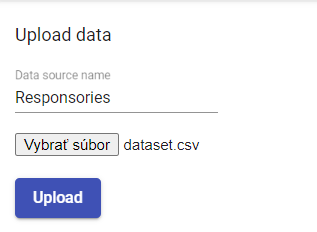
\includegraphics{udocs-upload-respon}
\caption{The upload form with the file \emph{dataset.csv} selected for upload. The new data source will have the name \emph{Responsories}.}
\label{fig:upload-ds}
\end{figure}

\begin{figure}[!h]
\centering
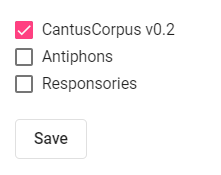
\includegraphics{udocs-ds-with-respon}
\caption{The uploaded data source automatically appears in the list.}
\label{fig:update-ds-respon}
\end{figure}

\section{Alignment}

It is possible to select a set of chants and have them be aligned using one of the methods described in section XXX. The alignment option is selected by clicking
on one of the buttons above the chant list after selecting the chants to be aligned. After doing so, the user is redirected to a page where the alignment result
is shown. In some cases, the alignment make take up to a minute to complete.

The alignment result is shown as a list of melodies. The melodies are either arranged in the same order as they were displayed in the chant list (in the case of
naive alignment) or in the order of similarity.

\begin{figure}[!h]
\centering
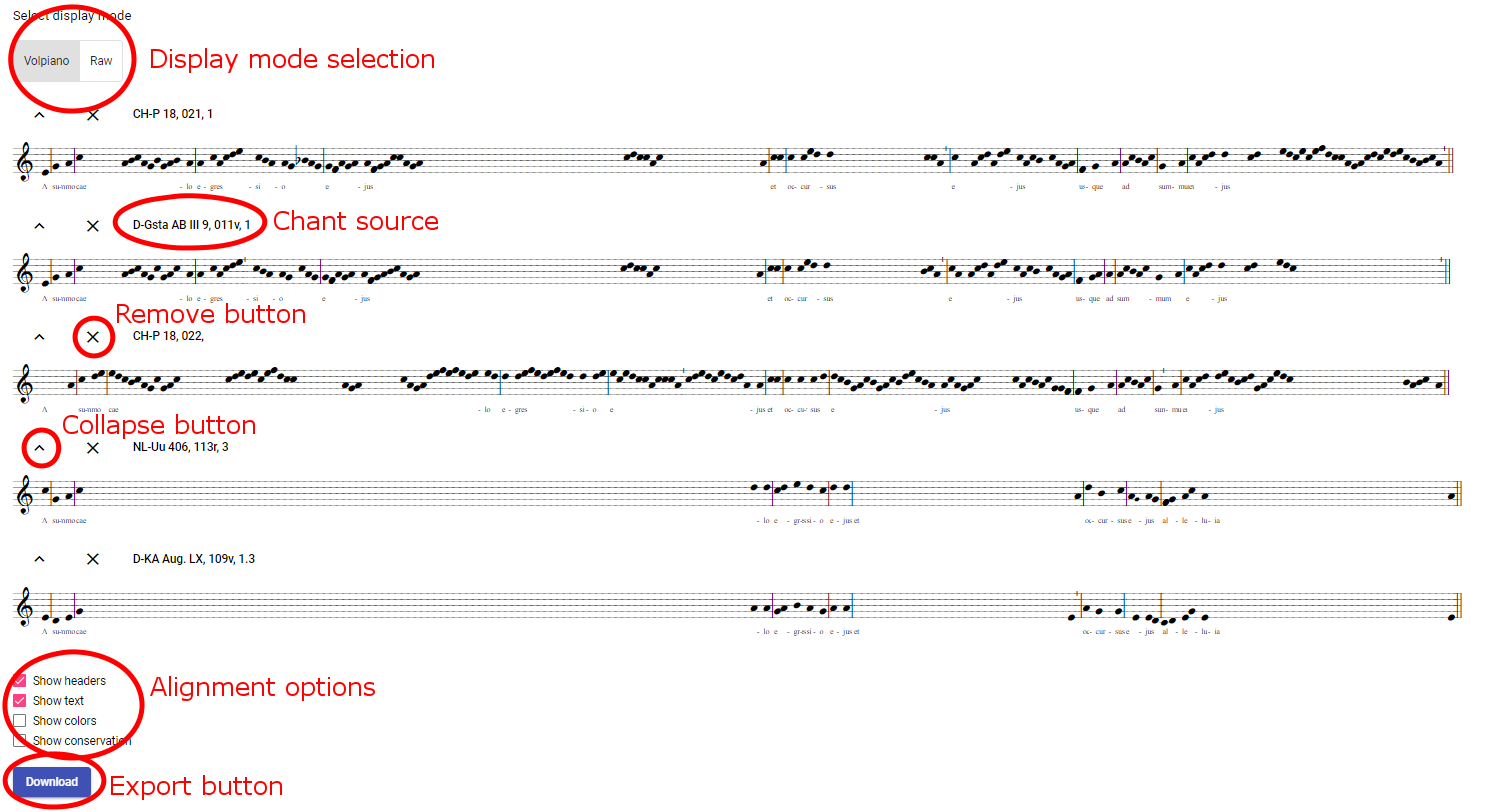
\includegraphics[scale=0.4]{udocs-alignment-basic-marked}
\caption{Result of the alignment.}
\label{fig:align-result}
\end{figure}

To show more information about each melody, the user can click on the chant source button by which each chant is identified. The same information as when navigating
to the chant's page is displayed. To hide the detail, click on the chant source button again.

\begin{figure}[!h]
\centering
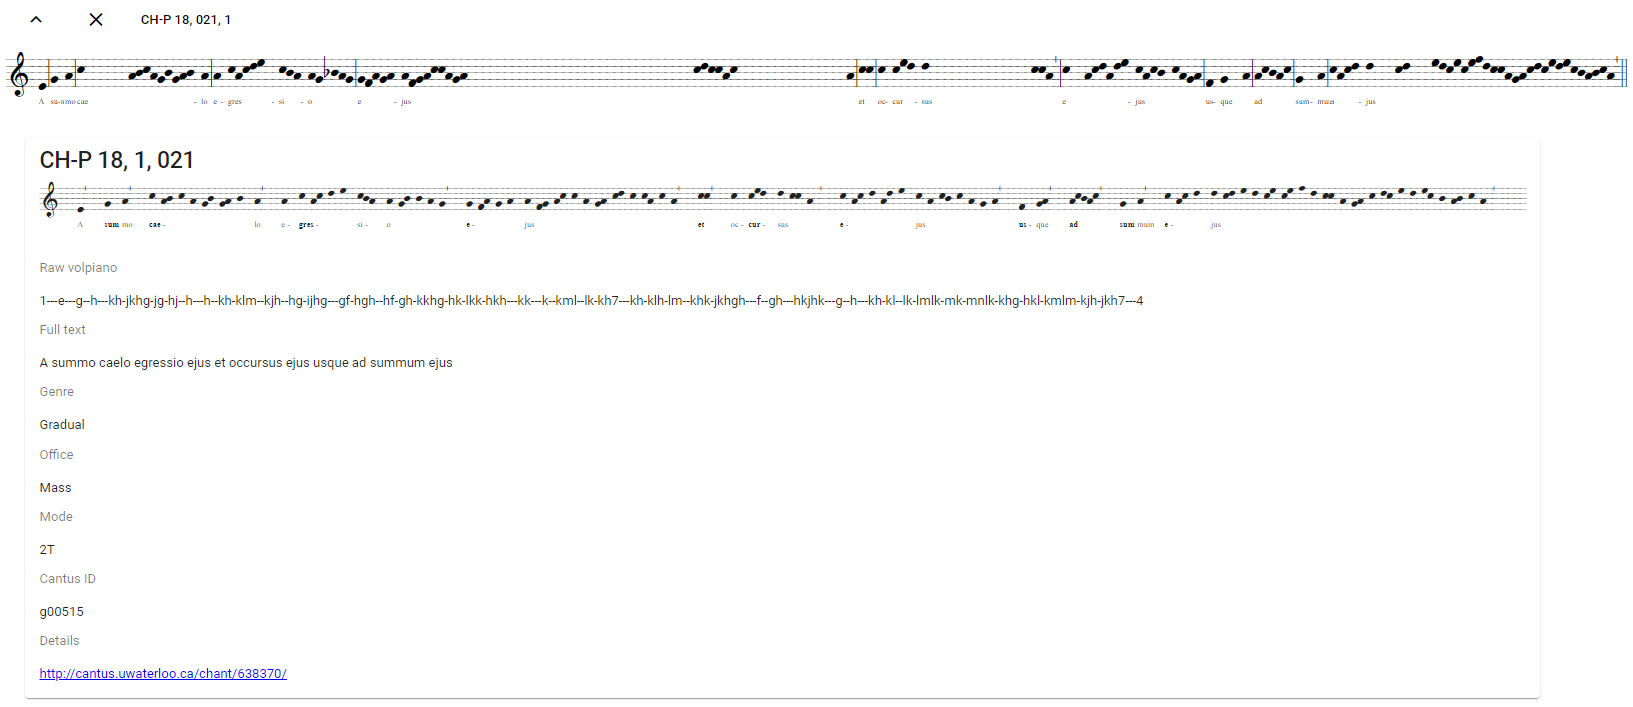
\includegraphics[scale=0.4]{udocs-alignment-detail}
\caption{Aligned melody with the chant information displayed.}
\label{fig:align-detail}
\end{figure}

If the user wishes to rearrange the displayed melodies, simply click anywhere close to a melody and drag it to another position.

\begin{figure}[!h]
\centering
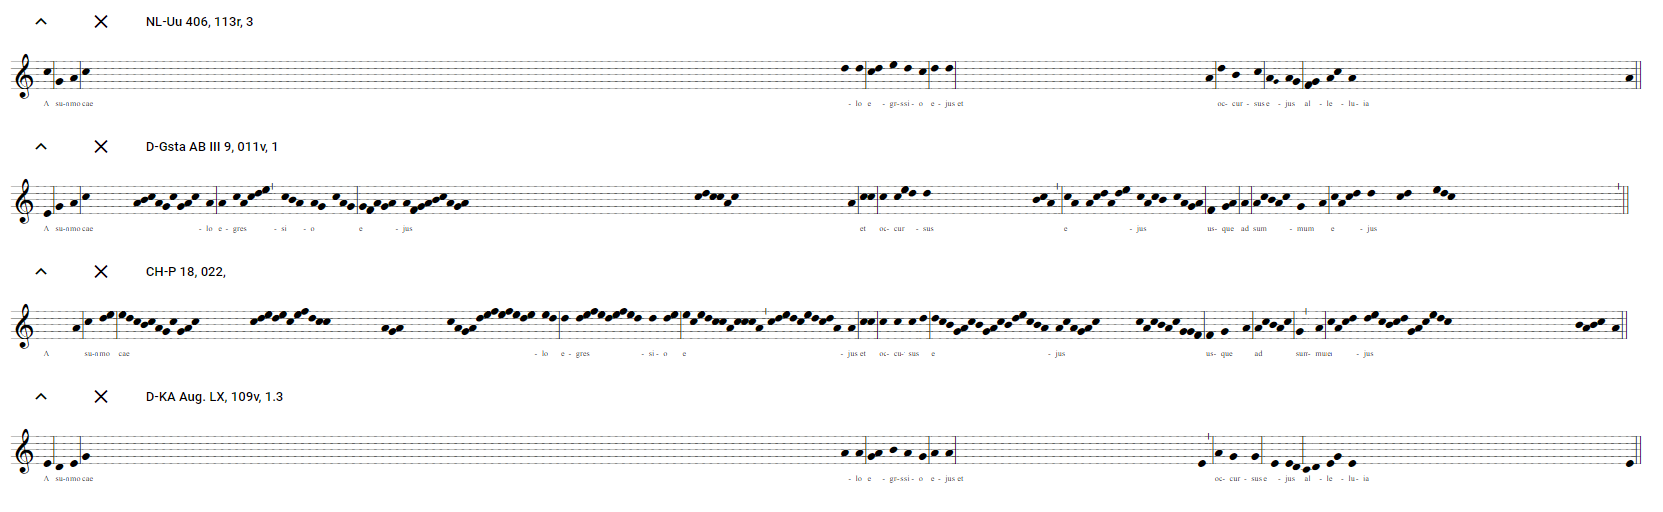
\includegraphics[scale=0.4]{udocs-alignment-rearrange}
\caption{Alignment after dragging and dropping the last melody. Compare to Figure \ref{fig:align-result}.}
\label{fig:align-rearrange}
\end{figure}

\subsection{Collapsing and deleting alignment}

After the alignment is shown, the user can choose to collapse the alignment (i.e. hide the notes) by clicking on the \emph{Collapse} button
in each melody's header or to remove it completely by clicking on the \emph{Remove button}. The chant can be uncollapsed by clicking
on the same button. However, removing the chant entirely is permanent. To get the removed chant back, the page needs to be reloaded.

\begin{figure}[!h]
\centering
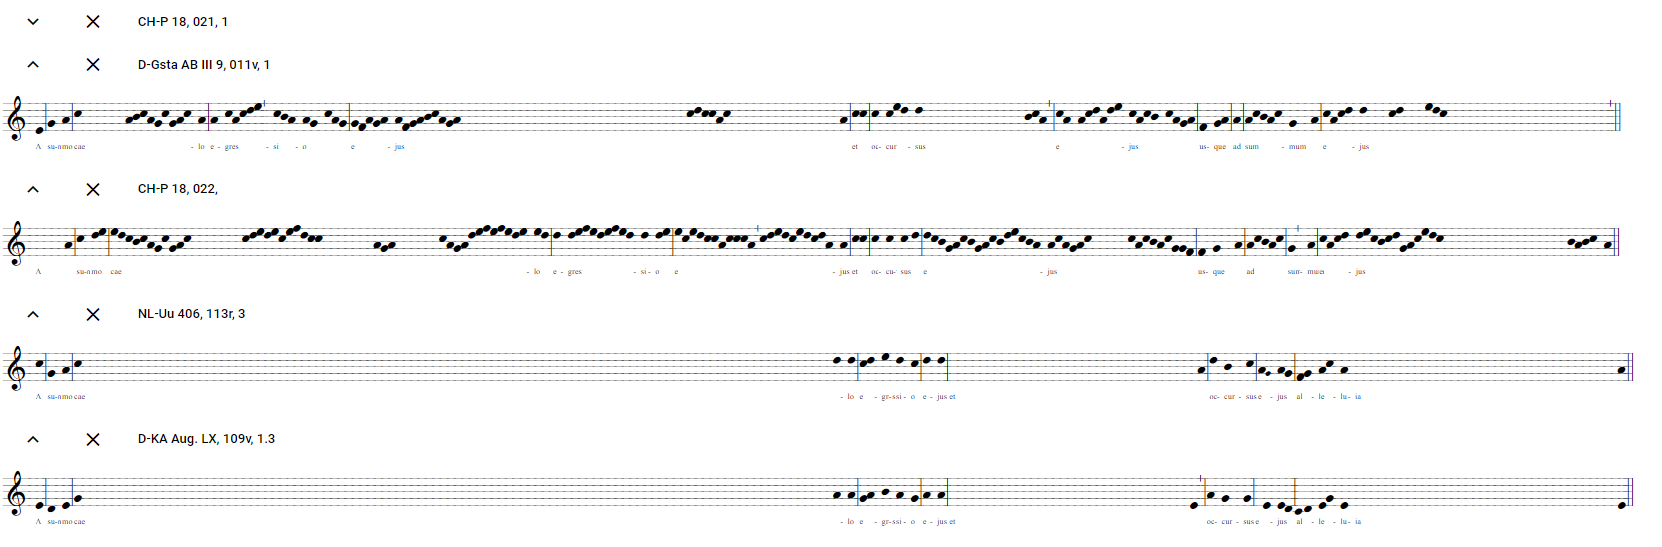
\includegraphics[scale=0.4]{udocs-alignment-collapsed}
\caption{The first chant is collapsed.}
\label{fig:align-collapsed}
\end{figure}

\begin{figure}[!h]
\centering
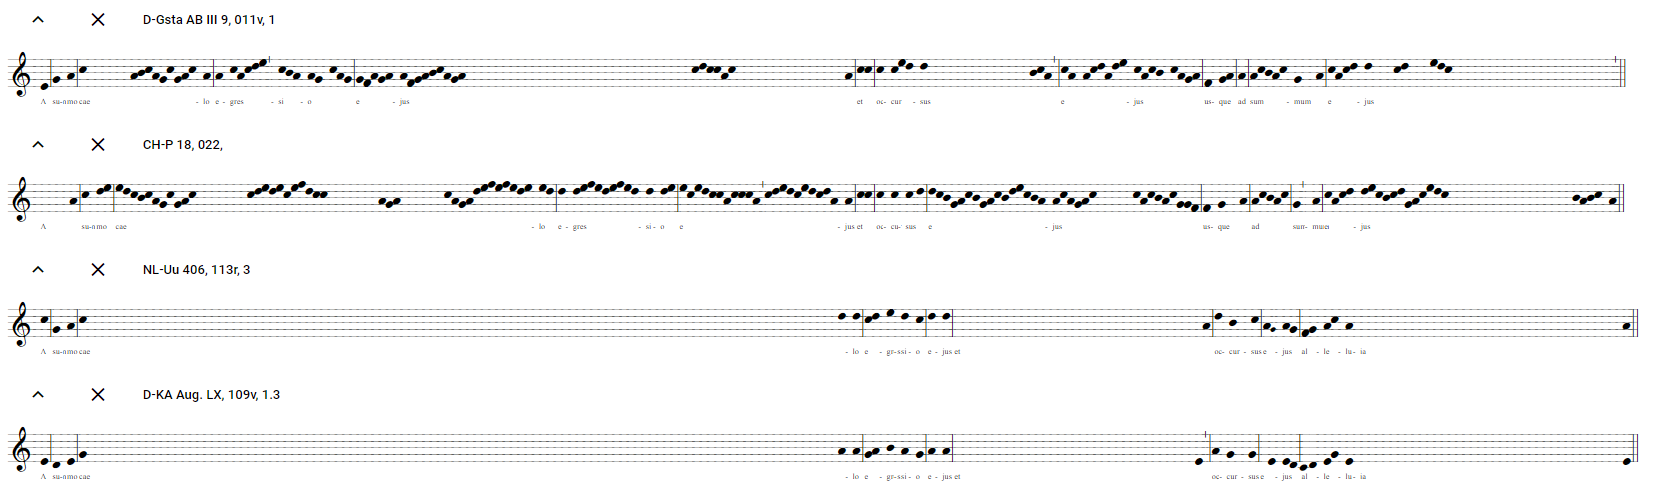
\includegraphics[scale=0.4]{udocs-alignment-deleted}
\caption{The first chant is removed. Compare to Figure \ref{fig:align-result}.}
\label{fig:align-removed}
\end{figure}

\subsection{Alignment display options}

Once the chants have been aligned, there exist several options to better show how they are aligned.

As the Volpiano font does not have characters of equal width, the notes that are actually aligned might not be shown as aligned. To see the
actual alignment, the user can change the display mode above the aligned melodies to \emph{Raw}, which shows the melodies as the encoded string
in a monopaced font.

\begin{figure}[!h]
\centering
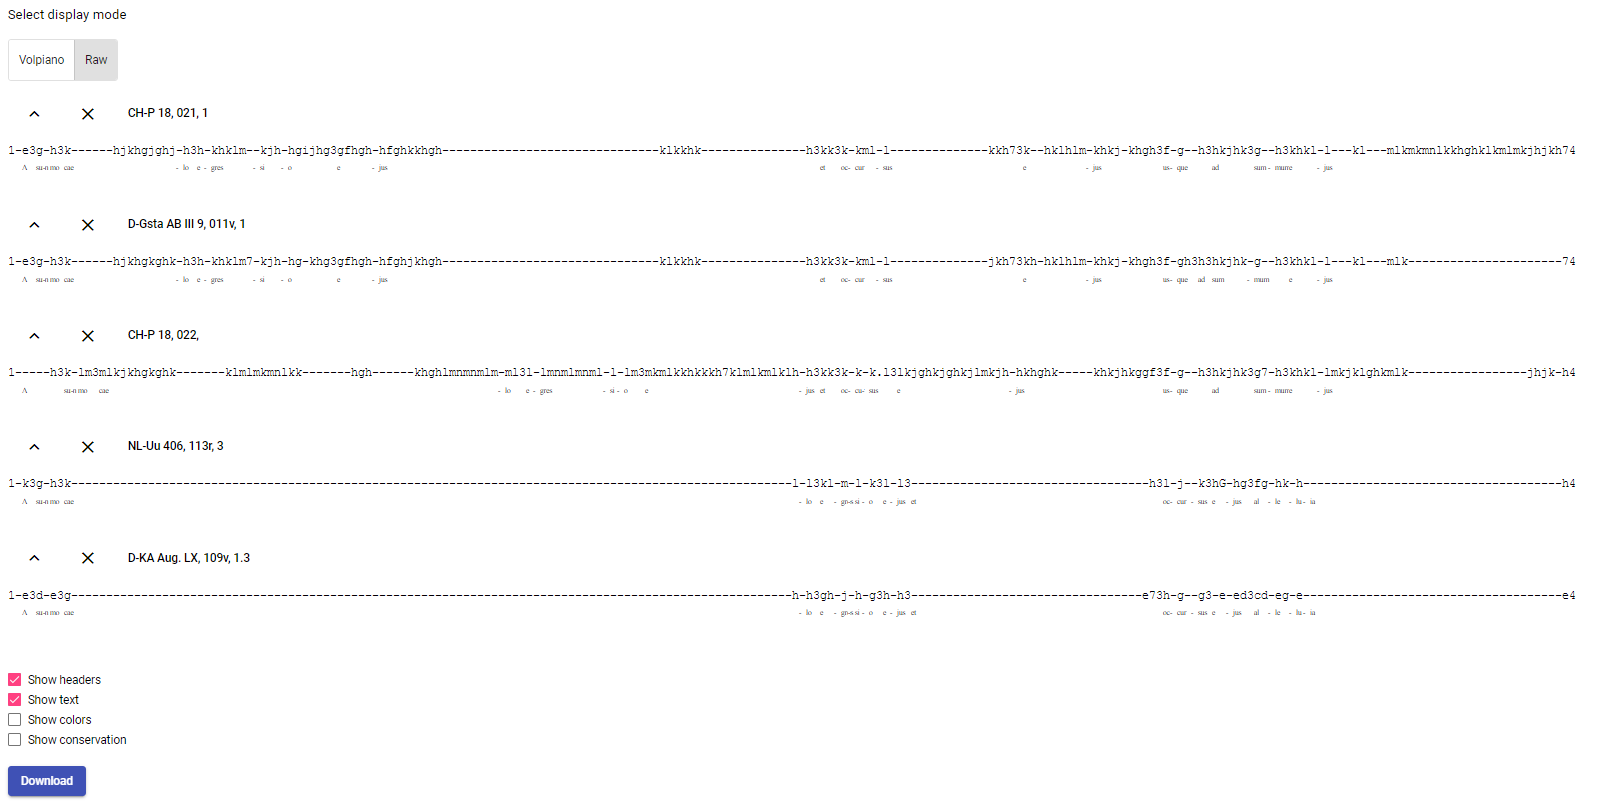
\includegraphics[scale=0.4]{udocs-alignment-raw}
\caption{Aligned melodies shown as the raw string.}
\label{fig:align-raw}
\end{figure}

To see the aligned sequences better, it is possible to remove the headers and the text independently by unclicking the corresponding boxes
in the alignment options.

\begin{figure}[!h]
\centering
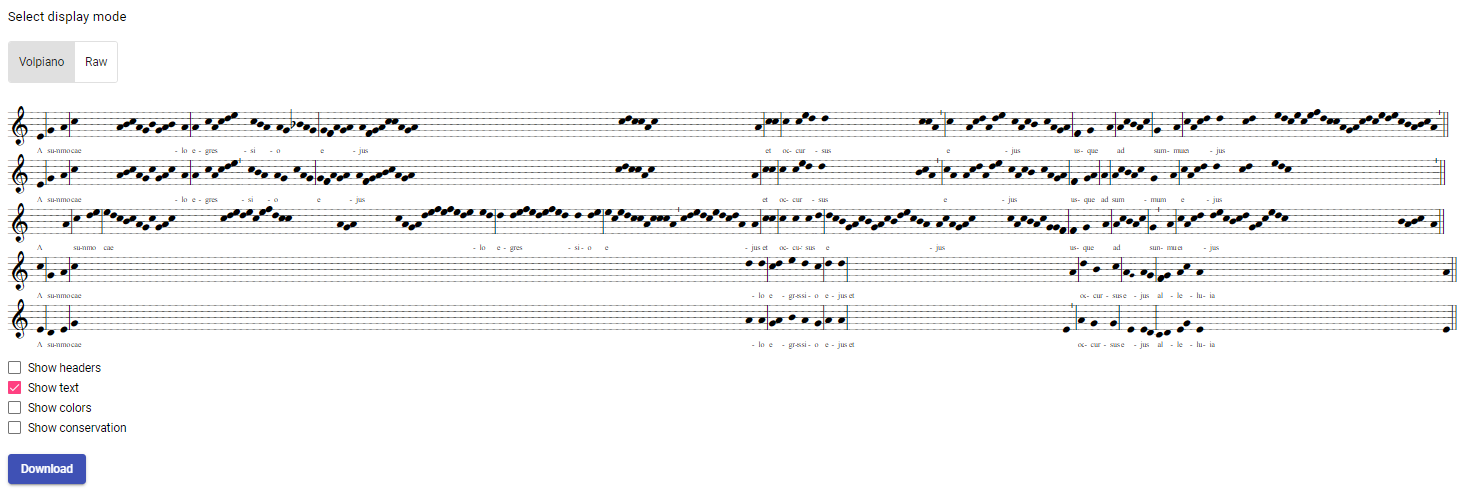
\includegraphics[scale=0.4]{udocs-alignment-no-headers}
\caption{The aligned melodies shown without headers.}
\label{fig:align-no-headers}
\end{figure}

\begin{figure}[!h]
\centering
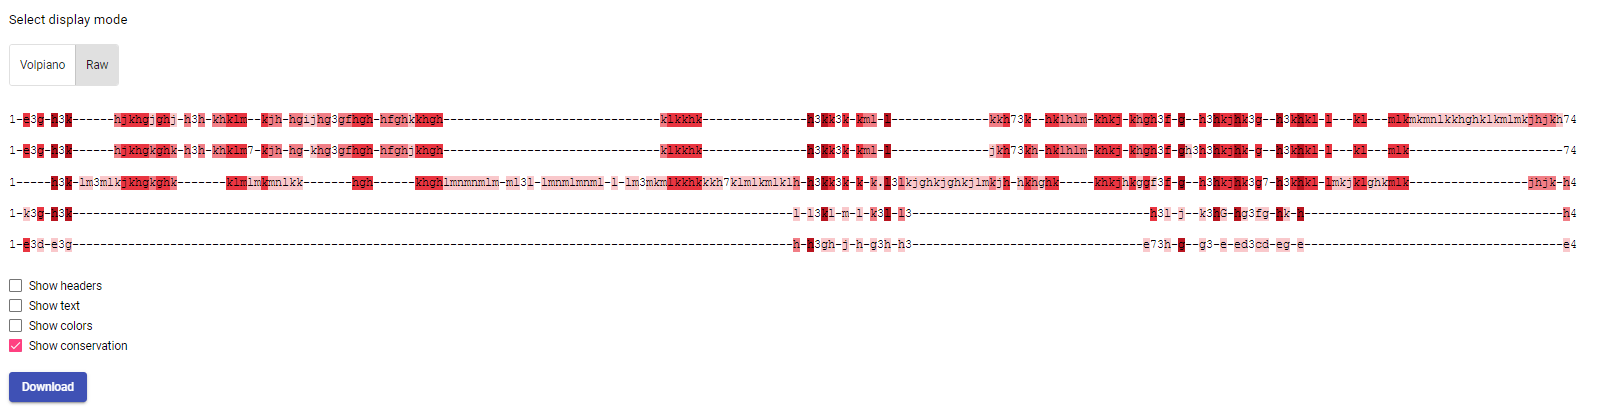
\includegraphics[scale=0.4]{udocs-alignment-no-headers-no-text}
\caption{The aligned melodies shown in \emph{Raw} mode without headers and text.}
\label{fig:align-no-text}
\end{figure}

It is possible to see how similar certain regions are. The first option is to color each note based on its absolute pitch. In the case of interval alignment,
this option may show different colors even though the intervals are the same.

\begin{figure}[!h]
\centering
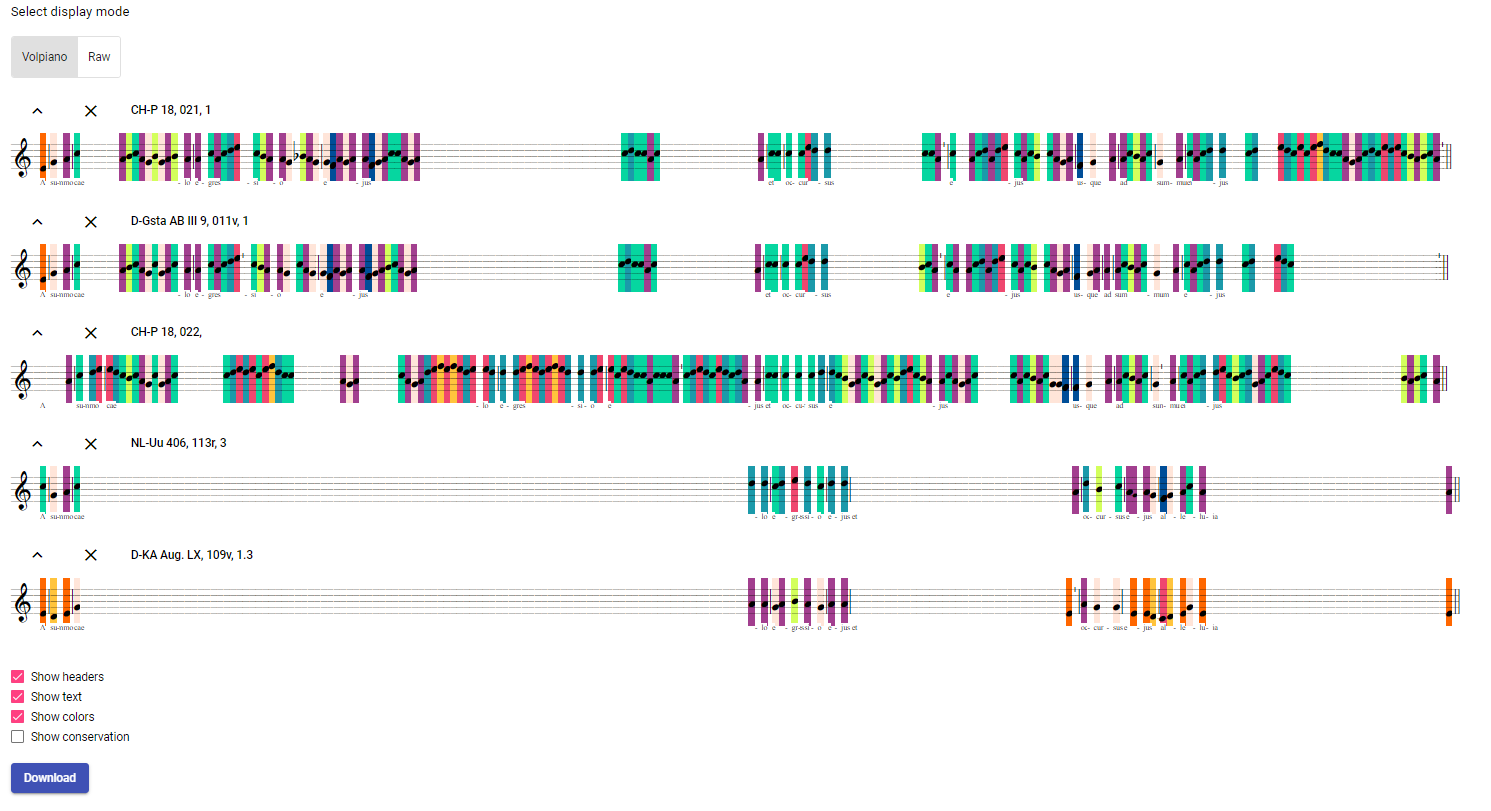
\includegraphics[scale=0.4]{udocs-alignment-vol-colors}
\caption{Aligned melodies with each note colored a different color.}
\label{fig:align-colors}
\end{figure}

The other option is to show the conservation profile, i.e. the proportion of the other chants sharing the same note or interval at the given position. This option will show
conservation profile corresponding to the intervals in the interval alignment option. Darker colors mean the position is more conserved, while lighter colors mean less conserved.
Using this option, it is possible to see how similar entire regions are.

\begin{figure}[!h]
\centering
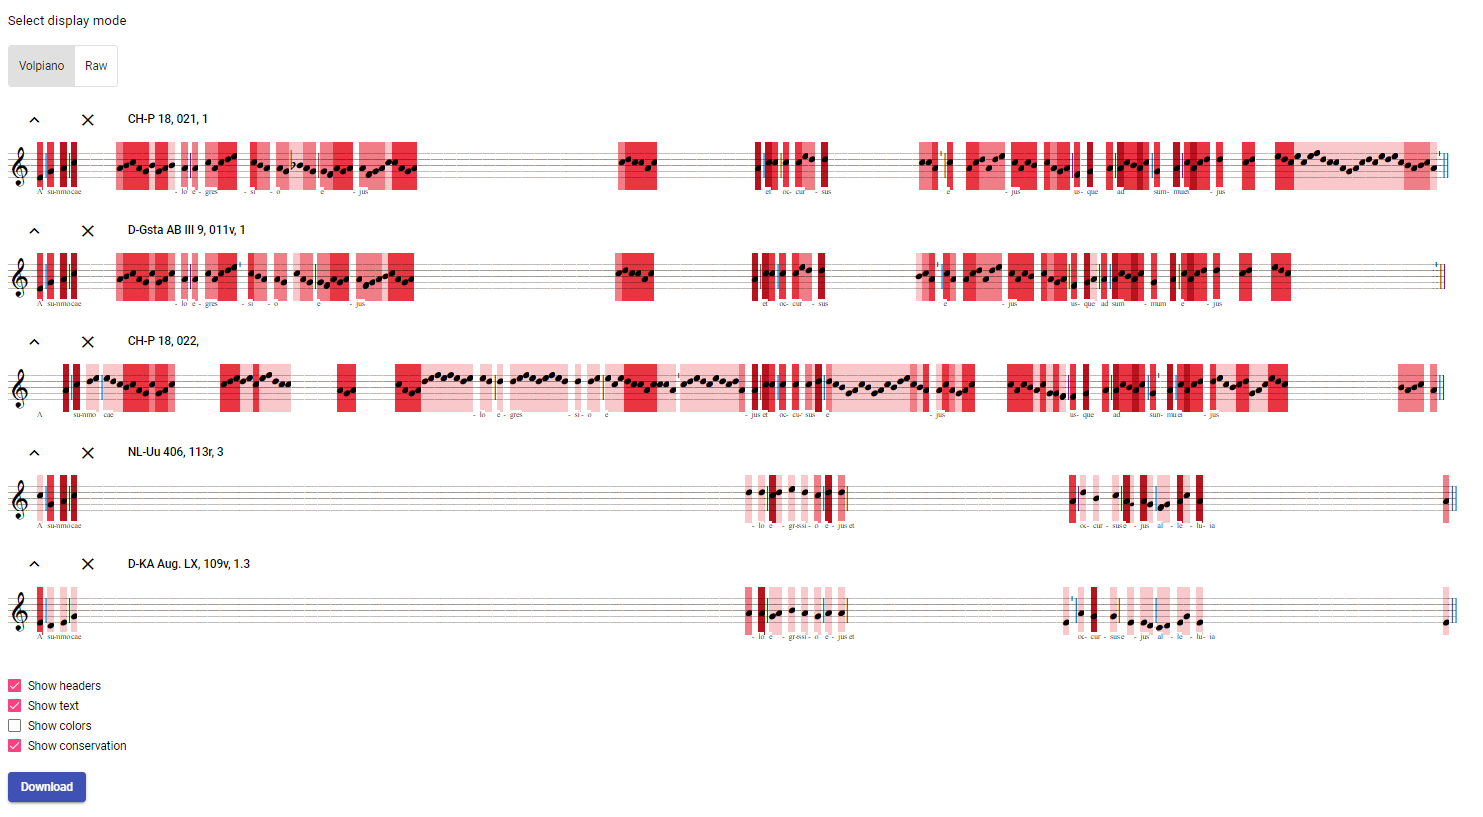
\includegraphics[scale=0.4]{udocs-alignment-vol-cons}
\caption{Aligned melodies with their conservation profile shown.}
\label{fig:align-cons}
\end{figure}

\subsection{Alignment export}

To export the aligned melodies, click the \emph{Download} button at the bottom of the page. The format of the file will be suitable to pass directly into MAFFT again. Each melody's
identifier is the string stored in the \emph{drupal\_path} field.

The melodies in the exported file will be either encoded as symbols corresponding to Volpiano characters in the case of naive and pitch alignment, or as symbols corresponding to intervals
in the case of interval alignment.

Only the unremoved melodies will be present in the file. Their order will be the same as the current order on the page.

\section{Dashboard}